\label{cap:analise}
\section{Tecnologias Utilizadas}

Neste trabalho, foram utilizadas algumas tecnologias e ferramentas que favoreceram e auxiliaram no desenvolvimento.

\subsection{Python 3}

Python é uma linguagem de programação de alto nível, com modelo de desenvolvimento aberto. \cite{python}. Surgiu em 1991 e tem se popularizado pela sua facilidade de aprendizado e simplicidade para implementação de scripts, análises e processamento de dados.

Este trabalho utilizou-se de uma das versões mais recentes da linguagem, que é a versão 3.5.3 (Setembro, 2017). 

\subsection{music21}

Uma biblioteca que contém diversas implementações que auxiliam no estudo da música. \cite{music21}.
Ela foi utilizada para auxiliar na leitura e formatação dos arquivos \textit{MIDI}, assim como o pré-processamento dos dados obtidos destes arquivos.

A biblioteca ainda provê implementação de alguns algoritmos que auxiliam na detecção do tom ou escala em que a composição foi escrita.

\subsection{Jupyter}

Trata-se de um projeto aberto e sem fins lucrativos que auxilia em computações científicas e de processameneto de dados e dispõe de uma interface interativa.


% ===============================================================
\section{Desenvolvimento}

A \textit{framework} desenvolvida é composta por três módulos principais:

\begin{itemize}
    \item \textit{probability.py}: Realiza as análises de frequência de uma composição musical para todos os modelos citados no \ref{cap:metodo}
    \item \textit{entropy.py}: Realiza os cálculos de entropia média e no instante para uma composição.
    \item \textit{graphs.ipynb}: \textit{Jupyter notebook} que gera os gráficos para as análises que serão mostradas a seguir
\end{itemize}

% ===============================================================
\section{Wave}

\begin{figure}[h]
\centering
\includegraphics[width=\textwidth]{Cap3/wave1}
\caption{Entropia de uma nota no instante para um trecho de \textit{Wave}}
\label{fig:wave1}
\end{figure}

\begin{figure}[h]
\centering
\includegraphics[width=\textwidth]{Cap3/wave2}
\caption{Entropia de uma nota e de notas vizinhas no instante para um trecho de \textit{Wave}}
\label{fig:wave2}
\end{figure}

\begin{figure}[h]
\centering
\includegraphics[width=\textwidth]{Cap3/compass_wave}
\caption{Média da Entropia instantânea de \textit{Wave} para todos os compassos}
\label{fig:compass_wave}
\end{figure}
Esta seção apresenta alguns resultados em relação à composição \textit{Wave}, de Tom Jobim, 1967. \cite{wave}

A figura \ref{fig:wave1} mostra os valores de entropia em cada instante de um treco da composição, isto é, a quantidade de informação transmitida nesse instante, em bits. Nesta análise, foi considerado o valor individual da nota.


A figura \ref{fig:wave2} insere na figura \ref{fig:wave1} o valor da entropia no instante ao se considerar a entropia condicional da nota daquele instante em relação a nota anterior. Pode-se notar que o formato das curvas muito se assemelham. Isto indica que a Informação Mútua é próxima de constante para o trecho exposto. Este resultado mostra como os intervalos utilizados pelo compositor muito se assemelham.


A figura \ref{fig:compass_wave} tenta encontrar algum padrão que se carrega por toda a música compasso a compasso. Trata-se da média da entropia ao decorrer do compasso, para todos os compassos da composição. Porém, o valor da entropia média por compasso é próxima de constante, o que nos indica que, apesar de uma informação mútua próxima a constante, os padrões que causam esse efeito se diferem compasso a compasso.

% ===============================================================
\section{Caprice No. 2}

\begin{figure}[h]
\centering
\includegraphics[width=\textwidth]{Cap3/paga1}
\caption{Entropia de uma nota no instante para um trecho de \textit{Caprice No. 2}}
\label{fig:paga1}
\end{figure}

\begin{figure}[h]
\centering
\includegraphics[width=\textwidth]{Cap3/paga2}
\caption{Entropia de uma nota e de notas vizinhas no instante para um trecho de \textit{Caprice No. 2}}
\label{fig:paga2}
\end{figure}

\begin{figure}[h]
\centering
\includegraphics[width=\textwidth]{Cap3/pagainfo}
\caption{Informação Mútua de duas notas vizinhas em \textit{Caprice No. 2} para um trecho}
\label{fig:pagainfo}
\end{figure}

\begin{figure}[h]
\centering
\includegraphics[width=\textwidth]{Cap3/paga3}
\caption{Média da Entropia instantânea de \textit{Caprice No. 2} para todos os compassos}
\label{fig:paga3}
\end{figure}

Esta seção apresenta alguns resultados em relação à composição \textit{Caprice No. 2} de Niccolò Paganini, 1817. \cite{caprice2}

A figura \ref{fig:paga1} mostra os valores de entropia em cada instante de um treco da composição, isto é, a quantidade de informação transmitida nesse instante, em bits. Nesta análise, foi considerado o valor individual da nota. Nota-se certos padrões em torno dos instantes $109$ e $121$. Esse efeito espelhado em torno desses instantes revela o formato desta música, em que o compositor leva a música a determinado ponto e volta da mesma maneira em se tratando de quantidade de informação transmitida.

A figura \ref{fig:paga2} insere na figura \ref{fig:paga1} o valor da entropia no instante ao se considerar a entropia condicional da nota daquele instante em relação a nota anterior. Pode-se notar que o formato das curvas e o valor delas muito se assemelham. Isto indica que a Informação Mútua é próxima de zero para o trecho exposto. Este resultado é melhor visto na figura \ref{fig:pagainfo}

A figura \ref{fig:paga3} mostra, assim como na seção anterior, a falta de padrões em relação aos compassos de toda a música.

% ===============================================================
\section{Evolução}


\begin{figure}[h]
\centering
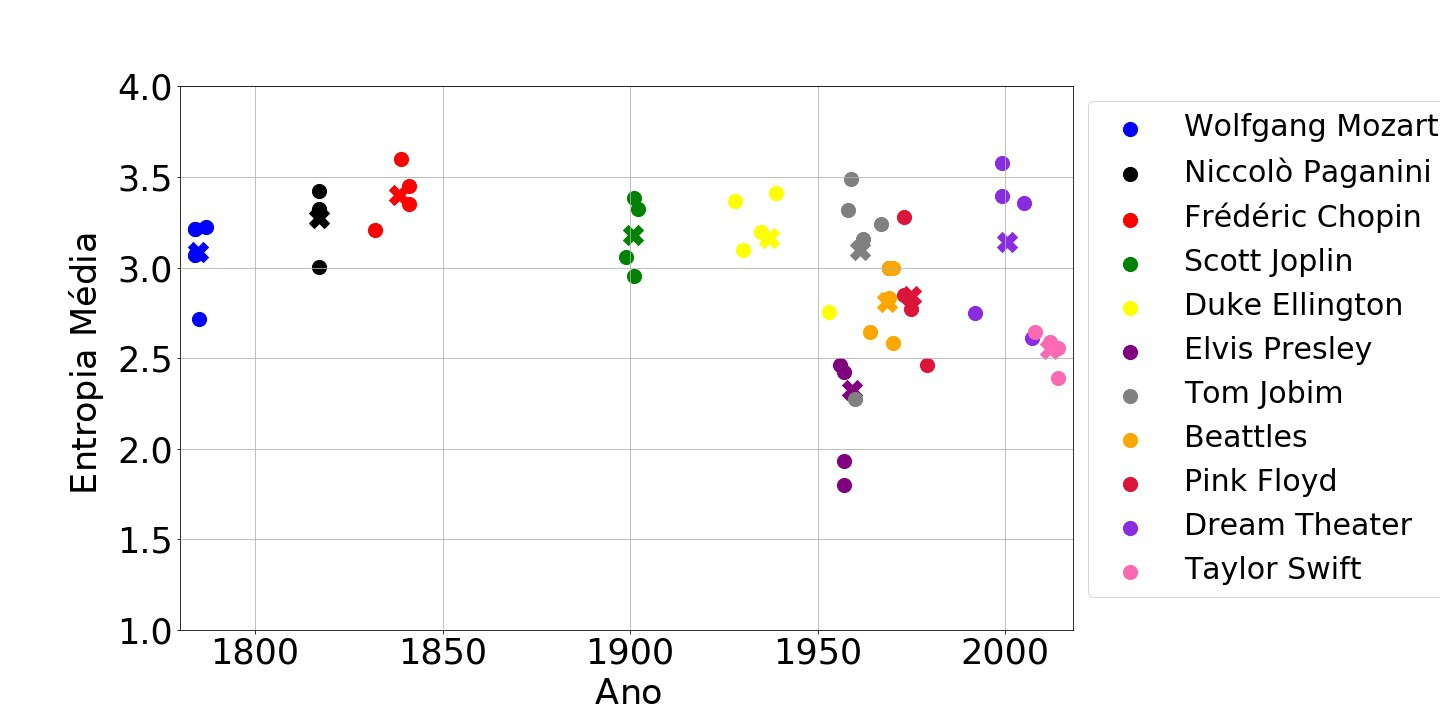
\includegraphics[width=\textwidth]{Cap3/evo.jpg}
\caption{Entropia Média de Composições ao longo dos anos}
\label{fig:evo}
\end{figure}

\begin{figure}[h]
\centering
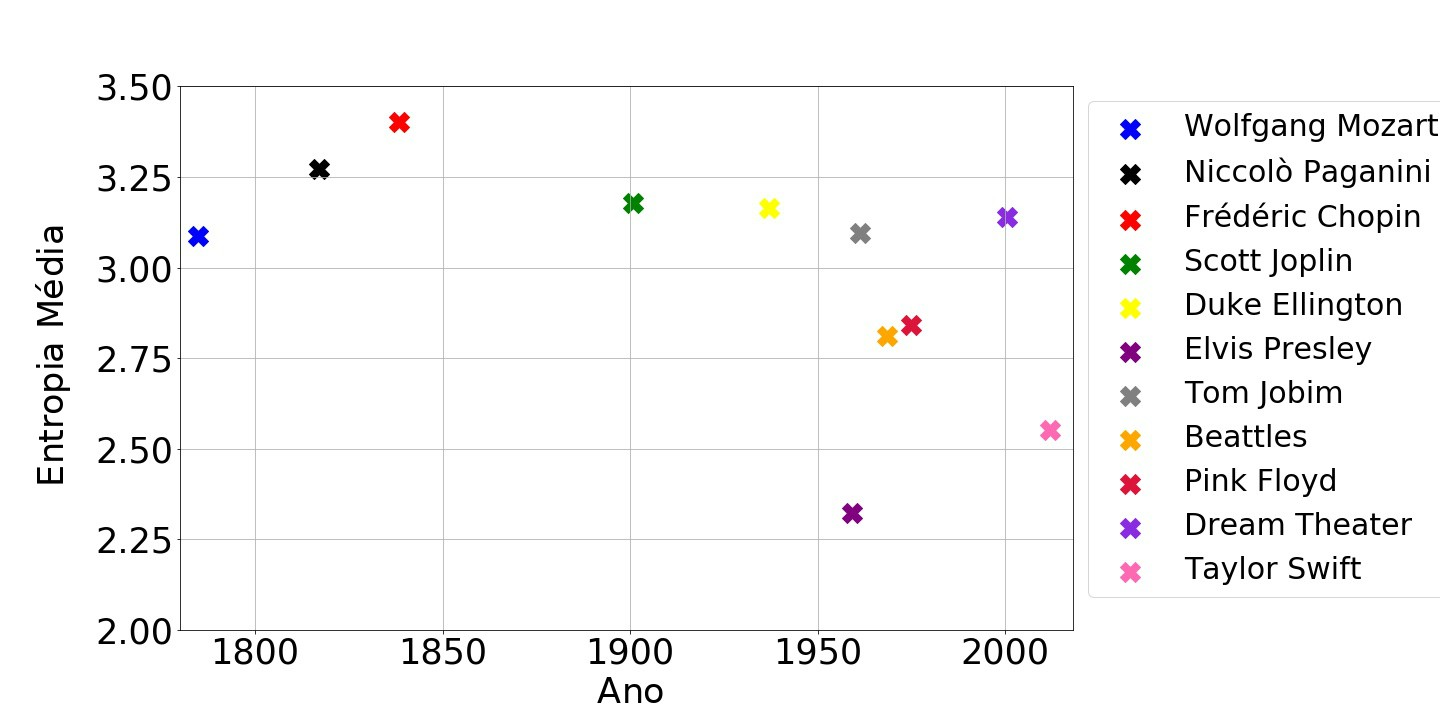
\includegraphics[width=\textwidth]{Cap3/marks2.jpg}
\caption{Entropia Média de Composições ao longo dos anos - Artistas}
\label{fig:artists}
\end{figure}

O objetivo desta seção é tentar retratar uma evolução da música internacional ao longo dos anos; desde artistas clássicos até os mais modernos. Foram utilizadas 52 composições de um total de 11 artistas e bandas. A composição mais antiga data de 1784 e a mais recente, de 2014. Os artistas utilizados, juntamente com os anos de atividade, são:

\begin{itemize}
    \item Wolfgang Amadeus Mozart (1761 - 1791) \cite{midiworld}
    \item Niccolò Paganini (1793 - 1840) \cite{midimelody}
    \item Frédéric François Chopin (1818 - 1849) \cite{midiworld}
    % \item Sergei Vasilievich Rachmaninoff (1877 - 1943) \cite{midiworld}
    \item Scott Joplin (1895 - 1917) \cite{trachtman}
    \item Duke Ellington (1914 - 1974) \cite{midimelody}
    \item Elvis Presley (1953 - 1977) \cite{midiworld}
    \item Antônio Carlos Jobim (1956 - 1994) \cite{wersi}
    \item The Beattles (1960 - 1970) \cite{midiworld}
    \item Pink Floyd (1965 - 1995, 2005, 2012 - 2014) \cite{midiworld}
    \item Dream Theater (1985 - Atualmente) \cite{freemidi}
    \item Taylor Swift (2004 - Atualmente) \cite{freemidi}
\end{itemize}
A figura \ref{fig:evo} mostra o valor médio de entropia de cada composição utilizando como evento as notas tocadas. O valor de cada composição está representado com um círculo e o valor médio por artista está representado com um $X$. 

A figura \ref{fig:artists} mostra o valor médio por artista e também apresenta uma escala mais precisa no eixo da entropia.

Nota-se uma pequena difereça entre os compositores mais clássicos (porção mais à esquerda) em relação aos artistas mais modernos, tendo os primeiros valores mais elevados de entropia. Nota-se também que as composições instrumentais apresentam entropia maior que aquelas as quais apenas a voz foi analisada (Voz: Todos a partir de Duke Ellington, com exceção de Pink Floyd e Dream Theater, que possui alguns solos de guitarra inclusos). Nota-se também que na porção mais moderna da linha do tempo, há uma opção maior em relação a entropia das composições. É importante notar, também, que esta análise deixa de considerar outras formas que o artista transmite informação, seja ela os \textit{riffs} base, efeitos na voz e letra.

Para uma comparação mais precisa, as tabelas de \ref{tab:mozart} até \ref{tab:taylor} mostram os valores de entropia calculados para cada uma das composições em cada um dos modelos já citatos no capítulo \ref{cap:metodo}.
% Please add the following required packages to your document preamble:
% \usepackage[table,xcdraw]{xcolor}
% If you use beamer only pass "xcolor=table" option, i.e. \documentclass[xcolor=table]{beamer}
\begin{table}[]
\centering
\caption{My caption}
\label{my-label}
\begin{tabular}{|c|c|c|c|c|c|}
\hline
\rowcolor[HTML]{9B9B9B} 
{\color[HTML]{FFFFFF} Composição}                                                                 & {\color[HTML]{FFFFFF} Ano} & {\color[HTML]{FFFFFF} H(Evento)} & {\color[HTML]{FFFFFF} H(Cond)} & {\color[HTML]{FFFFFF} H(Dist)} & {\color[HTML]{FFFFFF} H(Dur)} \\ \hline
\begin{tabular}[c]{@{}c@{}}Piano Sonata\\ No. 11\\ Movement 1\\ Theme and variations\end{tabular} & 1784                       &                                  &                                &                                &                               \\ \hline
\begin{tabular}[c]{@{}c@{}}Piano Sonata\\ No. 11\\ Movement 2\\ Menuetto and trio\end{tabular}    & 1784                       &                                  &                                &                                &                               \\ \hline
\begin{tabular}[c]{@{}c@{}}Piano Sonata\\ No. 11\\ Movement 3\\ Rondo alla turca\end{tabular}     & 1784                       &                                  &                                &                                &                               \\ \hline
Krebsgang                                                                                         & 1785                       &                                  &                                &                                &                               \\ \hline
\begin{tabular}[c]{@{}c@{}}Eine kleine\\ Nachtmusik\end{tabular}                                  & 1787                       &                                  &                                &                                &                               \\ \hline
\end{tabular}
\end{table}